\documentclass[aspectratio=43]{beamer}

% =========================================================
% PDFLATEX + TIENG VIET
% =========================================================
\usepackage[utf8]{inputenc}
\usepackage[T5]{fontenc}
\usepackage[vietnamese]{babel}
\usepackage{lmodern}

% =========================================================
% GOI CAN DUNG
% =========================================================
\usepackage{amsmath,amssymb,bm}
\usepackage{booktabs,array,multirow}
\usepackage{tikz}
\usetikzlibrary{arrows.meta,positioning,calc,shapes.geometric}
\usepackage{pgfplots}
\pgfplotsset{compat=1.18}
\usepackage{listings}

% =========================================================
% THEME
% =========================================================
\usetheme{Warsaw}

% GIỮ NGUYÊN các màu cũ để tcolorbox không bị thay đổi màu/thiết kế
\definecolor{mainblue}{RGB}{22,72,128}
\definecolor{softblue}{RGB}{236,244,252}
\definecolor{deepblue}{RGB}{12,45,90}
\definecolor{tealgreen}{RGB}{23,128,112}
\definecolor{softgreen}{RGB}{232,247,242}
\definecolor{warnred}{RGB}{180,55,55}
\definecolor{softred}{RGB}{255,239,239}
\definecolor{softyellow}{RGB}{255,248,225}
\definecolor{darkgray}{RGB}{45,45,45}

% ĐỊNH NGHĨA MÀU MỚI cho Header & Footer (Tone xanh tím giống hình 100%)
\definecolor{headleft}{RGB}{51,51,178}    % Màu nền ô trái (đậm)
\definecolor{headmid}{RGB}{160,160,215}   % Màu nền ô giữa / frametitle (vừa)
\definecolor{headright}{RGB}{200,200,230} % Màu nền ô phải (nhạt)

% Định nghĩa đúng 2 mã màu lấy từ ảnh mẫu
\definecolor{XanhTieuDe}{RGB}{0, 102, 34}    % Xanh lá đậm cho viền và tiêu đề
\definecolor{XanhNen}{RGB}{234, 245, 238}    % Xanh lá nhạt cho nền nội dung
\usepackage[most]{tcolorbox}
\newtcolorbox{baitapbox}[1]{
  colback=blue!5, colframe=blue!60!black, coltitle=white, 
  fonttitle=\bfseries, enhanced, title=#1,
}

\newtcolorbox{vidu}[1]{
  colback=XanhNen, 
  colframe=XanhTieuDe, 
  coltitle=white,
  fonttitle=\bfseries, 
  title=#1
}

\newtcolorbox{bode}[1]{ 
	enhanced, 
	colback=red!5!white, 
	colframe=red, 
	boxrule=0.5pt,
	arc=2mm,
	title={#1}, 
	fonttitle=\bfseries, 
	colbacktitle=red,
	attach boxed title to top left={xshift=5mm, yshift=-2.5mm}, 
	boxed title style={arc=3mm,, size=small}
}


% Áp dụng màu cho các thành phần cơ bản
%\setbeamercolor{title}{fg=deepblue}
\setbeamercolor{structure}{fg=headleft}
\setbeamercolor{normal text}{fg=darkgray,bg=white}
% \setbeamertemplate{itemize item}{\color{headleft}$\blacktriangleright$}
% \setbeamertemplate{itemize subitem}{\color{tealgreen}$\bullet$}
\setbeamertemplate{caption}[numbered]
% (Đã xóa dòng ẩn navigation symbols để thanh điều hướng hiện lên góc dưới phải giống ảnh)

% ---------------------------------------------------------
% 1. CẤU HÌNH HEADER (Thanh trên cùng - 2 ô chia đôi)
% ---------------------------------------------------------
\setbeamercolor{section in head/foot}{fg=white, bg=headleft}
\setbeamercolor{subsection in head/foot}{fg=black, bg=headright}

\setbeamertemplate{headline}
{
  \leavevmode%
  \hbox{%
  \begin{beamercolorbox}[wd=.5\paperwidth,ht=2.65ex,dp=1.5ex,right]{section in head/foot}%
    \usebeamerfont{section in head/foot}\insertsectionhead\hspace*{2ex}
  \end{beamercolorbox}%
  \begin{beamercolorbox}[wd=.5\paperwidth,ht=2.65ex,dp=1.5ex,left]{subsection in head/foot}%
    \usebeamerfont{subsection in head/foot}\hspace*{2ex}\insertsubsectionhead
  \end{beamercolorbox}}%
  \vskip0pt%
}

% ---------------------------------------------------------
% 2. CẤU HÌNH FRAMETITLE (Thanh tiêu đề slide)
% ---------------------------------------------------------
\setbeamercolor{frametitle}{fg=black, bg=headmid}

\setbeamertemplate{frametitle}
{
  \nointerlineskip
  \begin{beamercolorbox}[wd=\paperwidth,ht=3.2ex,dp=1.3ex,leftskip=.3cm,rightskip=.3cm]{frametitle}
    \usebeamerfont{frametitle}\insertframetitle
  \end{beamercolorbox}
}

% ---------------------------------------------------------
% 3. CẤU HÌNH FOOTER (Thanh dưới cùng - 3 ô)
% ---------------------------------------------------------
\setbeamercolor{author in head/foot}{fg=white, bg=headleft}
\setbeamercolor{title in head/foot}{fg=white, bg=headmid}
\setbeamercolor{date in head/foot}{fg=black, bg=headright}

\setbeamertemplate{footline}
{
  \leavevmode%
  \hbox{%
  \begin{beamercolorbox}[wd=.333333\paperwidth,ht=2.25ex,dp=1ex,center]{author in head/foot}%
    \usebeamerfont{author in head/foot}\insertshortauthor
  \end{beamercolorbox}%
  \begin{beamercolorbox}[wd=.333333\paperwidth,ht=2.25ex,dp=1ex,center]{title in head/foot}%
    \usebeamerfont{title in head/foot}\insertshorttitle
  \end{beamercolorbox}%
  \begin{beamercolorbox}[wd=.333333\paperwidth,ht=2.25ex,dp=1ex,right]{date in head/foot}%
    \usebeamerfont{date in head/foot}\insertframenumber{} / \inserttotalframenumber\hspace*{2ex}
  \end{beamercolorbox}}%
  \vskip0pt%
}

% =========================================================
% TCOLORBOX STYLE - GIU MOI NOI DUNG TRONG TCOLORBOX
% =========================================================
\tcbset{
  enhanced,
  boxrule=0pt,
  arc=2mm,
  left=1.7mm,
  right=1.7mm,
  top=1.2mm,
  bottom=1.2mm,
  fonttitle=\bfseries,
  coltitle=white
}

\newtcolorbox{defbox}[1]{
  title={#1},
  colback=softblue,
  colframe=mainblue,
  colbacktitle=mainblue
}

\newtcolorbox{keybox}[1]{
  title={#1},
  colback=softgreen,
  colframe=tealgreen,
  colbacktitle=tealgreen
}

\newtcolorbox{warnbox}[1]{
  title={#1},
  colback=softred,
  colframe=warnred,
  colbacktitle=warnred
}

\newtcolorbox{notebox}[1]{
  title={#1},
  colback=softyellow,
  colframe=orange!75!black,
  colbacktitle=orange!75!black
}

% Hộp "Lưu ý" được dùng ở phần BDF nhưng chưa được định nghĩa, khiến slide không
% biên dịch được. Định nghĩa lại theo đúng kiểu notebox.
\newtcolorbox{luuy}[1]{
  title={#1},
  colback=softyellow,
  colframe=orange!75!black,
  colbacktitle=orange!75!black
}

% =========================================================
% LENH TAT
% =========================================================
\newcommand{\R}{\mathbb{R}}
\newcommand{\C}{\mathbb{C}}
\newcommand{\norm}[1]{\left\lVert #1 \right\rVert}
\newcommand{\abs}[1]{\left| #1 \right|}
\newcommand{\dd}{\mathrm{d}}

% =========================================================
% THONG TIN BAO CAO
% =========================================================
\title[Phương pháp đa bước tuyến tính]{Phương pháp đa bước tuyến tính}
\subtitle{Sai số, tính nhất quán, ổn định và sự hội tụ}
\author{L. T. Nhân, D. T. H. Yến, N. H. Tú}
\institute{Trường Đại học Khoa học Tự nhiên, ĐHQG-HCM}
\date{\today}

\AtBeginSection[]{
  \begin{frame}
    \tableofcontents[currentsection]
  \end{frame}
}

\begin{document}
% =========================================================
\begin{frame}
  \titlepage
\end{frame}

\begin{frame}
\tableofcontents
\end{frame}

% =========================================================
\section{Mở đầu và kiến thức chuẩn bị}

\begin{frame}
\begin{baitapbox}{Phạm vi báo cáo}
Báo cáo tập trung vào khung lý thuyết của \textbf{phương pháp đa bước tuyến tính} khi giải bài toán giá trị đầu
\[
  y'(t)=f(t,y(t)),\qquad y(t_0)=y_0.
\]
\end{baitapbox}
\begin{itemize}
  \item Thiết lập công thức đa bước và các đa thức đặc trưng.
  \item Phân tích sai số, tính nhất quán, 0-ổn định và hội tụ.
  \item Trình bày định lý tương đương Dahlquist.
  \item Khảo sát họ BDF bậc thấp và minh họa bằng ví dụ số.
\end{itemize}
% \vspace{0.15cm}
% \begin{tcolorbox}[title={Các mục đã lược bỏ}, colback=softred, colframe=warnred, colbacktitle=warnred]
% 1.1.2, 1.2, 1.3 và 4.2.
% \end{tcolorbox}
\end{frame}
\subsection*{Khai triển Taylor}
\begin{frame}
\begin{baitapbox}{Công thức Taylor}
Giả sử $y\in C^{m+1}([t_0,T])$. Với $t,t+h\in [t_0,T]$:
\[
 y(t+h)=y(t)+hy'(t)+\frac{h^2}{2!}y''(t)+\cdots+\frac{h^m}{m!}y^{(m)}(t)+R_m(t),
\]
\[
 R_m(t)=\frac{h^{m+1}}{(m+1)!}y^{(m+1)}(\xi),\qquad \xi \in (\min(t,t+h),\max(t,t+h)).
\]
\end{baitapbox}
\begin{tcolorbox}[title={Vai trò trong phương pháp đa bước}, colback=softgreen, colframe=tealgreen, colbacktitle=tealgreen]
Khai triển Taylor giúp xây dựng công thức xấp xỉ đạo hàm và đánh giá \textbf{sai số chặt cụt cục bộ}. Các hệ số được chọn để triệt tiêu các bậc thấp của $h$.
\end{tcolorbox}
\end{frame}
\subsection*{Định lý tồn tại nghiệm Picard}
\begin{frame}

\begin{baitapbox}{Định lý Picard - Lindelöf}
    \begin{enumerate}
        \item Nếu $f$ liên tục trên miền hình chữ nhật:
        \[
        R = \{(t,y): t_0 \le t \le T_{max}\}
        \]
        \item Hàm số $f$ bị chặn trên miền hình chữ nhật:
        \[
        M_0 =max\{|f(t;y)|:(t;y) \in R\}
        \]
        và hơn nữa $M_0(T_{max} - t_0) \le y_M$
        \item Nếu $f$ liên tục theo $t$ và Lipschitz theo biến $y$, tức tồn tại $L > 0$ sao cho
        \[
        \|f(t, u) - f(t, v)\| \le L\|u - v\|, \qquad \forall t \in [t_0, T], \quad \forall u, v \in \mathbb{R}^d,
        \]
    \end{enumerate}
   
\end{baitapbox}
% \begin{itemize}
%   \item Định lý bảo đảm bài toán được đặt chỉnh trước khi áp dụng phương pháp số.
%   \item Trong phân tích hội tụ, giả thiết Lipschitz giúp chặn sự lan truyền sai số toàn cục.
% \end{itemize}
\end{frame}

\begin{frame}
     Nếu $f$ thỏa mãn các điều kiện trên thì tồn tại $\epsilon > 0$ sao cho bài bài toán
    \[
    y'(t) = f(t, y(t)), \qquad t \in [t_0, T_{max}], \qquad y(t_0) = y_0
    \]
    có duy nhất nghiệm $y(t)$ trong đoạn $[t_0-\epsilon;t_0+\epsilon]$
\end{frame}
\subsection*{Phương trình sai phân tuyến tính hệ số hằng}
\begin{frame}
\begin{baitapbox}{Phương trình sai phân tuyến tính}
Xét phương trình sai phân tuyến tính cấp $k$:
\[
 \alpha_k y_{n+k}+\alpha_{k-1}y_{n+k-1}+\cdots+\alpha_0y_n=0,
 \qquad \alpha_k\ne0.
\]
Tìm nghiệm dạng $y_n=\zeta^n$ thu được đa thức đặc trưng:
\[
 \rho(\zeta)=\alpha_k\zeta^k+\alpha_{k-1}\zeta^{k-1}+\cdots+\alpha_0=0.
\]
\end{baitapbox}
\begin{tcolorbox}[title={Ý nghĩa}, colback=softgreen, colframe=tealgreen, colbacktitle=tealgreen]
Cấu trúc nghiệm của sai phân quyết định khả năng sai số bị chặn hay bị khuếch đại khi $n\to\infty$.
\end{tcolorbox}
\end{frame}

% \begin{frame}{Điều kiện nghiệm từ sai phân}
% \begin{columns}[T]
% \column{0.52\textwidth}
% Nếu $\zeta_i$ là nghiệm của $\rho(\zeta)=0$:
% \begin{itemize}
%   \item Nghiệm đơn đóng góp thành phần $C_i\zeta_i^n$.
%   \item Nghiệm bội $m_i$ đóng góp các thành phần $n^r\zeta_i^n$, $r=0,\ldots,m_i-1$.
% \end{itemize}
% \column{0.48\textwidth}
% \begin{tcolorbox}[title={Điều kiện bị chặn}, colback=softgreen, colframe=tealgreen, colbacktitle=tealgreen]
% Dãy nghiệm bị chặn khi mọi nghiệm thỏa $\abs{\zeta_i}\le 1$ và mọi nghiệm trên đường tròn đơn vị $\abs{\zeta_i}=1$ đều là nghiệm đơn.
% \end{tcolorbox}
% \end{columns}
% \end{frame}
\subsection*{Phép nội suy đa thức Lagrange}
\begin{frame}
\begin{baitapbox}{Đa thức nội suy Lagrange}
Cho $n+1$ điểm dữ liệu $(x_0,y_0),\ldots,(x_n,y_n)$. Đa thức nội suy bậc không vượt quá $n$ có dạng
\[
 P(x)=\sum_{i=0}^{n} y_i L_i(x),
\]
trong đó
\[
 L_i(x)=\prod_{\substack{j=0\\j\ne i}}^{n}\frac{x-x_j}{x_i-x_j}.
\]
\end{baitapbox}
\begin{tcolorbox}[title={Liên hệ với BDF}, colback=softgreen, colframe=tealgreen, colbacktitle=tealgreen]
BDF được xây dựng bằng cách nội suy các giá trị nghiệm quá khứ và lấy đạo hàm của đa thức nội suy tại điểm mới.
\end{tcolorbox}
\end{frame}

% =========================================================
\section{Phương pháp đa bước tuyến tính và sai số}

\begin{frame}
\begin{baitapbox}{Rời rạc hóa miền thời gian}
Chia đoạn $[t_0,T]$ thành $N$ đoạn con:
\[
 h=\frac{T-t_0}{N},\qquad t_n=t_0+nh,\qquad n=0,1,\ldots,N.
\]
Ký hiệu:
\[
 y(t_n): \text{ nghiệm chính xác},\qquad Y_n\approx y(t_n): \text{ nghiệm số}.
\]
Sai số toàn cục tại nút $t_n$:
\[
 e_n=y(t_n)-Y_n.
\]
\end{baitapbox}
\end{frame}
\subsection*{Phương pháp đa bước tuyến tính tổng quát}
\begin{frame}
\begin{baitapbox}{Phương pháp đa bước tuyến tính $k$ bước}
Một phương pháp đa bước tuyến tính $k$ bước có dạng
\[
 \sum_{j=0}^{k}\alpha_jY_{n+j}
 =h\sum_{j=0}^{k}\beta_j f(t_{n+j},Y_{n+j}),
\]
trong đó
\[
 \alpha_k\ne 0,\qquad |\alpha_0|+|\beta_0|>0.
\]
\end{baitapbox}
\begin{tcolorbox}[title={Ý tưởng}, colback=softgreen, colframe=tealgreen, colbacktitle=tealgreen]
Tái sử dụng thông tin từ nhiều bước trước để tính bước mới. Hiệu quả tính toán cao hơn, nhưng cần giá trị khởi động và kiểm soát ổn định chặt chẽ hơn.
\end{tcolorbox}
\end{frame}
\subsection*{Đa thức đặc trưng thứ nhất và thứ hai}
\begin{frame}
\begin{baitapbox}{Đa thức đặc trưng}
Với phương pháp
\[
 \sum_{j=0}^{k}\alpha_jY_{n+j}=h\sum_{j=0}^{k}\beta_j f(t_{n+j},Y_{n+j}),
\]
ta gắn hai đa thức:
\[
 \rho(\zeta)=\sum_{j=0}^{k}\alpha_j\zeta^j,
 \qquad
 \sigma(\zeta)=\sum_{j=0}^{k}\beta_j\zeta^j.
\]
\end{baitapbox}
\begin{itemize}
  \item $\rho(\zeta)$: quyết định 0-ổn định qua điều kiện nghiệm.
  \item $\sigma(\zeta)$: tham gia điều kiện nhất quán và sai số chặt cụt.
\end{itemize}
\end{frame}
\subsection*{Phân loại phương pháp đa bước tuyến tính }
\begin{frame}

\begin{baitapbox}{Phương pháp hiện}
Nếu $\beta_k=0$, $Y_{n+k}$ tính trực tiếp từ dữ liệu quá khứ.
\[
Y_{n+k}= -\sum_{j=0}^{k-1}\frac{\alpha_j}{\alpha_k}Y_{n+j}
+h\sum_{j=0}^{k-1}\frac{\beta_j}{\alpha_k}f_{n+j}.
\]
\end{baitapbox}

\begin{baitapbox}{Phương pháp ẩn}
Nếu $\beta_k\ne0$, $Y_{n+k}$ xuất hiện trong $f(t_{n+k},Y_{n+k})$, cần giải phương trình ẩn:
\[
Y_{n+k} = h\cdot\frac{\beta_k}{\alpha_k}f(t_{n+k};Y_{n+k}) + \dots + \text{Thành phần quá khứ}
\]
\end{baitapbox}

% \begin{tcolorbox}[title={Bài toán khởi động}, colback=softred, colframe=warnred, colbacktitle=warnred]
% LMM $k$ bước cần $Y_0,Y_1,\ldots,Y_{k-1}$, trong khi IVP chỉ cho $Y_0$. Thường dùng RK4 hoặc phương pháp một bước bậc cao để tạo mồi.
% \end{tcolorbox}
\end{frame}
\subsection*{Toán tử sai phân tuyến tính}
\begin{frame}
\begin{baitapbox}{Toán tử sai phân tuyến tính}
Với hàm trơn $y(t)$, định nghĩa
\[
 L[y](t;h)=\sum_{j=0}^{k}\left[\alpha_jy(t+jh)-h\beta_jy'(t+jh)\right].
\]
Khai triển Taylor cho ta
\[
 L[y](t;h)=C_0y(t)+C_1hy'(t)+C_2h^2y''(t)+\cdots+C_qh^qy^{(q)}(t)+\cdots.
\]
\end{baitapbox}
\begin{tcolorbox}[title={Bậc chính xác}, colback=softgreen, colframe=tealgreen, colbacktitle=tealgreen]
Phương pháp có bậc $p$ nếu
\[
 C_0=C_1=\cdots=C_p=0,\qquad C_{p+1}\ne0.
\]
\end{tcolorbox}
\end{frame}

\begin{frame}
\begin{baitapbox}{Hệ số Taylor của toán tử sai phân}
\[
 C_0=\sum_{j=0}^{k}\alpha_j,
\]
\[
 C_1=\sum_{j=0}^{k}(j\alpha_j-\beta_j),
\]
\[
 C_q=\sum_{j=0}^{k}\left(\frac{j^q}{q!}\alpha_j-\frac{j^{q-1}}{(q-1)!}\beta_j\right),\qquad q\ge 2.
\]
Độ chính xác của LMM có thể kiểm tra trực tiếp từ các hệ số $\alpha_j,\beta_j$.
\end{baitapbox}
\end{frame}

% \begin{frame}{Các nguồn sai số trong tính toán số}
% \begin{center}
% \begin{tikzpicture}[node distance=1.1cm, every node/.style={font=\small}, box/.style={rounded corners, draw=mainblue, fill=softblue, thick, align=center, minimum width=3.7cm, minimum height=0.85cm}]
% \node[box] (local) {Sai số cục bộ};
% \node[box, right=1.0cm of local] (trunc) {Sai số chặt cụt};
% \node[box, below=0.9cm of local] (round) {Sai số làm tròn};
% \node[box, below=0.9cm of trunc] (start) {Sai số khởi động};
% \node[draw=tealgreen, fill=softgreen, thick, rounded corners, align=center, minimum width=4cm, minimum height=1cm, below right=0.65cm and -1.35cm of round] (global) {Sai số toàn cục\\$e_n=y(t_n)-Y_n$};
% \draw[-{Latex}, thick] (local) -- (global);
% \draw[-{Latex}, thick] (trunc) -- (global);
% \draw[-{Latex}, thick] (round) -- (global);
% \draw[-{Latex}, thick] (start) -- (global);
% \end{tikzpicture}
% \end{center}
% \begin{tcolorbox}[title={Mục tiêu}, colback=softgreen, colframe=tealgreen, colbacktitle=tealgreen]
% Chứng minh $\max_n\norm{e_n}\to0$ khi $h\to0$ dưới các điều kiện thích hợp.
% \end{tcolorbox}
% \end{frame}
\subsection*{Sai số phương pháp đa bước}
\begin{frame}
    \begin{baitapbox}{Sai số chặt cụt}
        Sai số chặt cụt của phương pháp đa bước tuyến tính được định nghĩa bởi:
        \[
        T_n = \frac{ \sum_{j=0}^{k} \left[ \alpha_j y(t_{n+j})  -h  \beta_j f(t_{n+j}, y(t_{n+j}))\right]}{h \sum_{j=0}^{k} \beta_j} = \frac{\mathcal{L}[y](t_n; h)}{h \sigma(1)}
        \]
    \end{baitapbox}
    Xét bài toán (IVP) và công thức tổng quát của phương pháp đa bước:
    \[
        y'=f(t;y) \qquad \sum_{j=0}^{n} \alpha_j Y_{n+j}  =h  \sum_{j=0}^{n}\beta_j f(t_{n+j}, Y_j)
    \]
    Phân dư khi xấp xĩ bằng khai triển Tayor:
    \[
        R_n = \sum_{j=0}^{k} \alpha_j y(t_{n+j})  -h  \sum_{j=0}^{k}\beta_j f(t_{j}, y(t_{n+j}))
    \]
\end{frame}

\begin{frame}
    Bằng công thứ sai phân tuyến tính ta có phần dư có thể được viết lại:
    \[
        R_n = \mathcal{L}[y](t_n; h) = \sum \alpha_j y(t) + \left(\sum j\alpha_j -\sum \beta_j\right) h y'(t) + \mathcal{O}({h^2})
    \]
        Ta thu phóng phần dư này một cách thích hợp để $T_n$ tương tự như $y'-f(t;y)$, trong trường hợp này ta chuẩn hóa bằng chia các vế cho $h\sum\beta_j$:
    \[
        T_n = \frac{R_n}{h\sum \beta_j} = \frac{\mathcal{L}[y](t_n; h)}{h\sigma(1)}
    \]
\end{frame}


% =========================================================
\section{Nhất quán, ổn định và hội tụ}
\subsection*{Tính nhất quán và điều kiện đại số}
\begin{frame}
\begin{baitapbox}{Tính nhất quán}
Phương pháp đa bước tuyến tính được gọi là \textbf{nhất quán} nếu sai số chặt cụt tiến về $0$ đồng đều khi $h\to0$:
\[
 \lim_{h\to0}\max_{0\le n\le N}\norm{T_n}=0.
\]
\end{baitapbox}
\begin{tcolorbox}[title={Ý nghĩa}, colback=softgreen, colframe=tealgreen, colbacktitle=tealgreen]
Khi lưới đủ mịn, công thức sai phân phải mô phỏng đúng phương trình vi phân ban đầu.
\end{tcolorbox}
\end{frame}

\begin{frame}
\begin{baitapbox}{Điều kiện đại số tính nhất quán}
Nhắc lại:
\[
 \rho(\zeta)=\sum_{j=0}^{k}\alpha_j\zeta^j,
 \qquad
 \sigma(\zeta)=\sum_{j=0}^{k}\beta_j\zeta^j.
\]
Một LMM nhất quán khi và chỉ khi
\[
 \rho(1)=0,
 \qquad
 \rho'(1)=\sigma(1).
\]
\end{baitapbox}
\begin{itemize}
  \item $\rho(1)=0$: phương pháp chính xác với nghiệm hằng.
  \item $\rho'(1)=\sigma(1)$: phương pháp chính xác với nghiệm tuyến tính.
\end{itemize}
\end{frame}

\subsection*{Tính $0-$ổn định}

\begin{frame}
\begin{baitapbox}{Tính $0-$ổn định và định lý $0-$ổn định}
Phương pháp được gọi là 0-ổn định nếu tồn tại $K>0$ độc lập với $h$ sao cho với hai dãy nghiệm $\{Y_n\}$ và $\{Z_n\}$ sinh bởi cùng phương pháp,
\[
 |Y_n-Z_n|\le K\max_{0\le j\le k-1}|Y_j-Z_j|,
 \qquad n\ge k.
\]
\end{baitapbox}
\begin{itemize}
  \item 0-ổn định đo khả năng kiểm soát nhiễu nhỏ từ dữ liệu khởi động.
  \item Đây là điều kiện bắt buộc để sai số không bị khuếch đại vô hạn.
\end{itemize}
\end{frame}

\begin{frame}

\begin{baitapbox}{Định lý về $0-$ổn định}
LMM là 0-ổn định khi và chỉ khi mọi nghiệm $\zeta_i$ của $\rho(\zeta)=0$ thỏa \textit{điều kiện nghiệm}:
\begin{itemize}
    \item Tất cả nghiệm đều nằm trong hoặc trên đường tròn đơn vị: $|\zeta_i|\le1$
    \item Nếu nghiệm nằm trên đường tròn đơn vị $|\zeta_i|=1$ thì đó là \textit{nghiệm đơn}
\end{itemize}
\end{baitapbox}

% \begin{center}
% \begin{tikzpicture}[scale=1.05]
% \draw[->] (-1.45,0)--(1.65,0) node[right] {$\Re z$};
% \draw[->] (0,-1.25)--(0,1.25) node[above] {$\Im z$};
% \draw[mainblue, thick] (0,0) circle (1);
% \fill[tealgreen] (1,0) circle (2pt) node[below right] {$z=1$};
% \fill[warnred] (1.35,0.35) circle (2pt) node[right] {$|z|>1$};
% \node[mainblue] at (0,-1.5) {Đường tròn đơn vị};
% \end{tikzpicture}
% \end{center}

\end{frame}
\subsection*{Sự hội tụ phương pháp đa bước}
\begin{frame}
\begin{baitapbox}{Sự hội tụ}
Phương pháp đa bước tuyến tính được gọi là hội tụ nếu với mọi IVP thỏa các giả thiết đặt chỉnh,
\[
 \displaystyle\lim_{h\to 0 , \\ nh=t-t_0}Y_n=y(t),
 \qquad t\in[t_0,T].
\]
\end{baitapbox}
\begin{baitapbox}{Bậc hội tụ}
Phương pháp hội tụ bậc $p$ nếu tồn tại $C>0$ độc lập với $h,n$ sao cho
\[
 \max_{0\le n\le N}|y(t_n)-Y_n|\le Ch^p=O(h^p).
\]
\end{baitapbox}
\end{frame}
\subsection*{Định lý hội tụ chính}
\begin{frame}
\begin{baitapbox}{Định lý tương đương Dahlquist}
Đối với phương pháp đa bước tuyến tính có hệ số hằng và dữ liệu khởi đầu tương thích:
\[
 \boxed{\text{Hội tụ}\quad \Longleftrightarrow\quad \text{Nhất quán} + \text{0-ổn định}.}
\]
\end{baitapbox}
\begin{itemize}
  \item Tính nhất quán bảo đảm sai số sinh ra trong từng bước đủ nhỏ.
  \item Tính 0-ổn định bảo đảm sai số không bị khuếch đại khi lan truyền.
  \item Kết hợp hai điều kiện cho ta hội tụ toàn cục.
\end{itemize}
\end{frame}

\begin{frame}{Ý tưởng chứng minh: chiều thuận}
\begin{enumerate}
  \item Xét bài toán $y'=0$, $y(0)=0$. Công thức trở thành sai phân thuần nhất:
  \[
    \alpha_kY_{n+k}+\cdots+\alpha_0Y_n=0.
  \]
  Hội tụ buộc nghiệm sai phân không được bùng nổ $\Rightarrow$ thỏa điều kiện nghiệm $\Rightarrow$ 0-ổn định.
  \item Xét các bài toán thử $y'=0$ và $y'=1$. Từ hội tụ suy ra
  \[
    \rho(1)=0,
    \qquad
    \rho'(1)=\sigma(1).
  \]
  Do đó phương pháp nhất quán.
\end{enumerate}
\end{frame}

\begin{frame}{Ý tưởng chứng minh: chiều đảo}
\begin{itemize}
  \item Nhất quán cho sai số chặt cụt $T_n\to0$ khi $h\to0$.
  \item 0-ổn định cho phép chặn nghiệm của phương trình sai phân sai số.
  \item Dùng bổ đề Gronwall rời rạc để suy ra
  \[
    |e_n|\le C\left(\delta(h)+\max_m |T_m|\right),
  \]
  trong đó $\delta(h)$ là sai số khởi động.
  \item Nếu dữ liệu khởi động tương thích, $\delta(h)\to0$, nên $e_n\to0$.
\end{itemize}
\begin{tcolorbox}[title={Kết luận}, colback=softgreen, colframe=tealgreen, colbacktitle=tealgreen]
Nghiệm số hội tụ về nghiệm chính xác trên toàn đoạn khảo sát.
\end{tcolorbox}
\end{frame}

% =========================================================
\section{Họ phương pháp BDF}
\subsection*{Xây dựng và khảo sát một số BDF}
\begin{frame}
\begin{baitapbox}{Xây dựng họ vi phân lùi BDF}
BDF dùng đa thức nội suy qua các giá trị nghiệm đã biết và giá trị mới, sau đó xấp xỉ đạo hàm tại điểm mới.
\[
 y'(t_{n+1})\approx q'(t_{n+1}).
\]
Công thức tổng quát theo sai phân lùi:
\[
 \sum_{j=1}^{k}\frac{1}{j}\nabla^jY_{n+1}=hf(t_{n+1},Y_{n+1}).
\]
\end{baitapbox}
\begin{tcolorbox}[title={Đặc điểm}, colback=softgreen, colframe=tealgreen, colbacktitle=tealgreen]
BDF là phương pháp \textbf{ẩn}, thường có tính ổn định tốt và phù hợp với các bài toán cứng.
\end{tcolorbox}
\end{frame}

\begin{frame}{BDF1: Euler ẩn}
\begin{baitapbox}{Công thức BDF1}
Với $k=1$:
\[
 Y_{n+1}-Y_n=hf(t_{n+1},Y_{n+1}).
\]

Khai triển Taylor quanh $t_{n+1}$:
\[
 \frac{y_{n+1}-y_n}{h}=y'(t_{n+1})-\frac{h}{2}y''(t_{n+1})+O(h^2).
\]
\end{baitapbox}
\begin{tcolorbox}[title={Kết luận}, colback=softgreen, colframe=tealgreen, colbacktitle=tealgreen]
BDF1 có bậc chính xác $p=1$.
\end{tcolorbox}
\end{frame}

\begin{frame}
\begin{baitapbox}{Công thức BDF2}
Với $k=2$, lấy đạo hàm đa thức nội suy bậc hai tại $t_{n+2}$:
\[
 \frac{3}{2}Y_{n+2}-2Y_{n+1}+\frac{1}{2}Y_n=hf(t_{n+2},Y_{n+2}).
\]

Khai triển Taylor quanh $t_{n+2}$:
\begin{align*}
    \Leftrightarrow \frac{3y_{n+2} - 4y_{n+1} + y_n}{2h} &= y'(t_{n+2}) - \frac{1}{3}h^2 y'''(t_{n+2}) \\
    &\quad + \frac{1}{4}h^3 y^{(4)}(t_{n+2}) + \mathcal{O}(h^4)
\end{align*}


\end{baitapbox}
\begin{tcolorbox}[title={Kết luận}, colback=softgreen, colframe=tealgreen, colbacktitle=tealgreen]
BDF2 có bậc chính xác $p=2$.
\end{tcolorbox}
\end{frame}

\begin{frame}
\begin{baitapbox}{Công thức BDF3}
Với $k=3$, công thức BDF3 là
\[
 \frac{11}{6}Y_{n+3}-3Y_{n+2}+
 \frac{3}{2}Y_{n+1}-\frac{1}{3}Y_n
 =hf(t_{n+3},Y_{n+3}).
\]

Khai triển Taylor quanh $t_{n+3}$:
\begin{align*}
    \Leftrightarrow \quad & \frac{11y_{n+3} - 18y_{n+2} + 9y_{n+1} - 2y_n}{6h} \\
    &= y'(t_{n+3}) - \frac{1}{4}h^3y^{(4)}(t_{n+3}) + O(h^4).
\end{align*}

\end{baitapbox}
\begin{tcolorbox}[title={Kết luận}, colback=softgreen, colframe=tealgreen, colbacktitle=tealgreen]
BDF3 có bậc chính xác $p=3$.
\end{tcolorbox}
\end{frame}

\begin{frame}
\begin{baitapbox}{Tính nhất quán của họ BDF}
BDF $k$ bước có bậc chính xác
\[
 p=k,
 \qquad k\ge1.
\]
Vì một LMM có bậc $p\ge1$ thì nhất quán, suy ra mọi phương pháp BDF đều nhất quán.
\end{baitapbox}
\begin{luuy}{Lưu ý}
Phương pháp nhất quán chưa đủ để bảo đảm hội tụ. Ta vẫn phải kiểm tra điều kiện 0-ổn định.
\end{luuy}
\end{frame}

\begin{frame}
\begin{baitapbox}{Đa thức đặc trưng của BDF}
Đa thức đặc trưng của BDF $k$ bước có dạng
\[
 \rho(\zeta)=\sum_{j=1}^{k}\frac{1}{j}\zeta^{k-j}(\zeta-1)^j.
\]
Dùng phép biến đổi Möbius
\[
 \zeta=\frac{1}{1-z},
\]
thu được
\[
 \rho\left(\frac{1}{1-z}\right)=(1-z)^{-k}p(z),
 \qquad
 p(z)=\sum_{j=1}^{k}\frac{z^j}{j}.
\]
\end{baitapbox}
\end{frame}
\subsection*{Tính $0-$ổn định của BDF}
\begin{frame}
\begin{baitapbox}{Bổ đề về tính $0-$ổn định của BDF}
BDF 0-ổn định khi nghiệm của $p(z)$ nằm ngoài đĩa $|z-1|\le1$, trừ nghiệm biên đơn.
\end{baitapbox}
\begin{baitapbox}{Định lý}
Công thức BDF $k$ bước 0-ổn định với $k\le6$ và không 0-ổn định với $k\ge7$.
\end{baitapbox}
\end{frame}

% =========================================================
\section{Minh họa số: Ví dụ 1}
\subsection*{Ví dụ minh họa số}
\begin{frame}
\begin{vidu}{Phương pháp A}
Xét phương pháp đa bước hai bước
\[
 Y_{n+2}+4Y_{n+1}-5Y_n=h(4f_{n+1}+2f_n).
\]
Ta có
\[
 \rho(z)=z^2+4z-5,
 \qquad
 \sigma(z)=4z+2.
\]
\end{vidu}
\begin{columns}[T]
\column{0.5\textwidth}
\begin{tcolorbox}[title={Nhất quán}, colback=softgreen, colframe=tealgreen, colbacktitle=tealgreen]
\[
\rho(1)=1+4-5=0,
\]
\[
\rho'(1)=6=\sigma(1).
\]
\end{tcolorbox}
\column{0.5\textwidth}
\begin{tcolorbox}[title={Tính 0-ổn định}, colback=softred, colframe=warnred, colbacktitle=warnred]
\[
\rho(z)=(z-1)(z+5).
\]
 Có $|z|=5>1$.
\end{tcolorbox}
\end{columns}
\end{frame}

\begin{frame}
\begin{vidu}{Bài toán giá trị đầu}
Áp dụng phương pháp A cho IVP
\[
 y'(t)=-y(t),
 \qquad
 y(0)=1.
\]
Nghiệm chính xác:
\[
 y(t)=e^{-t}.
\]
\end{vidu}
\begin{tcolorbox}[title={Thay vào công thức}, colback=softgreen, colframe=tealgreen, colbacktitle=tealgreen]
Với $f_n= -Y_n$, công thức trở thành
\[
 Y_{n+2}+4(1-h)Y_{n+1}-(5+2h)Y_n=0.
\]
\end{tcolorbox}
\end{frame}

\begin{frame}{Phương trình đặc trưng của ví dụ}
\begin{tcolorbox}[title={Phương trình đặc trưng tương ứng}, colback=softgreen, colframe=tealgreen, colbacktitle=tealgreen]
\[
 \lambda^2+4(1-h)\lambda-(5+2h)=0.
\]
Khi $h$ nhỏ:
\[
 \lambda_1=1+O(h),
 \qquad
 \lambda_2=-5+O(h).
\]
\end{tcolorbox}
\begin{tcolorbox}[title={Nhận xét}, colback=softred, colframe=warnred, colbacktitle=warnred]
Vì một nghiệm có môđun xấp xỉ $5>1$, sai số nhỏ có thể bị khuếch đại rất nhanh qua từng bước lặp.
\end{tcolorbox}
\end{frame}
\begin{frame}
\begin{baitapbox}{Nghiệm tổng quát của sai phân}
Nghiệm tổng quát của sai phân có dạng
\[
 Y_n=C_1\lambda_1^n+C_2\lambda_2^n.
\]
Vì
\[
 |\lambda_2|\approx 5>1,
\]
thành phần $C_2\lambda_2^n$ bị khuếch đại theo cấp số nhân.
\end{baitapbox}
\begin{tcolorbox}[title={}, colback=softred, colframe=warnred, colbacktitle=warnred]
Tính nhất quán chỉ bảo đảm sai số sinh ra ở từng bước nhỏ. Nếu không 0-ổn định, các nhiễu nhỏ vẫn bị khuếch đại và làm nghiệm số phân kỳ.
\end{tcolorbox}
\end{frame}
\begin{frame}{Bảng nghiệm và sai số}
\begin{center}
\scriptsize
\begin{tabular}{cccc}
\toprule
$t$ & $y(t)$ & $Y_n$ & $|y(t)-Y_n|$ \\
\midrule
0.0 & $1.000000\times10^{0}$ & $1.000000\times10^{0}$ & $0$ \\
0.5 & $6.065307\times10^{-1}$ & $6.081996\times10^{-1}$ & $1.668921\times10^{-3}$ \\
1.0 & $3.678794\times10^{-1}$ & $-6.677259\times10^{0}$ & $7.045138\times10^{0}$ \\
2.0 & $1.353353\times10^{-1}$ & $-1.243391\times10^{8}$ & $1.243391\times10^{8}$ \\
4.0 & $1.831564\times10^{-2}$ & $-3.872979\times10^{22}$ & $3.872979\times10^{22}$ \\
6.0 & $2.478752\times10^{-3}$ & $-1.206376\times10^{37}$ & $1.206376\times10^{37}$ \\
\bottomrule
\end{tabular}
\end{center}
\begin{tcolorbox}[title={Nhận xét}, colback=softgreen, colframe=tealgreen, colbacktitle=tealgreen]
Sai số tăng rất nhanh, dù phương pháp đã nhất quán.
\end{tcolorbox}
\end{frame}

\begin{frame}{Đồ thị sai số tuyệt đối}
\begin{center}
\begin{tikzpicture}
\begin{semilogyaxis}[
    width=0.82\textwidth,
    height=0.50\textwidth,
    grid=both,
    xlabel={$t$},
    ylabel={$|y-Y|$},
    ymin=1e-4,ymax=1e40,
    xmin=0,xmax=6,
    tick label style={font=\scriptsize},
    label style={font=\small},
]
\addplot[mark=*, thick, mainblue] coordinates {
(0,1e-16)
(0.5,1.668921e-3)
(1.0,7.045138e0)
(2.0,1.243391e8)
(4.0,3.872979e22)
(6.0,1.206376e37)
};
\end{semilogyaxis}
\end{tikzpicture}
\end{center}
\end{frame}



% =========================================================
\section{Kiểm chứng bằng số}

\begin{frame}{Ranh giới $k \le 6$ của họ BDF, tính trực tiếp}
\begin{columns}[T]
\column{0.46\textwidth}
\footnotesize
Với mỗi $k$, hệ số BDF được dựng lại từ
\[
  \sum_{j=1}^{k}\tfrac{1}{j}\nabla^{j}Y_{n+k}=hf_{n+k},
\]
rồi giải số $\rho(z)=0$ và so $\max_i|z_i|$ với $1$.

\medskip
Ranh giới $k\le 6$ \textbf{không được giả định trước} — nó hiện ra từ chính vị trí
nghiệm của đa thức đặc trưng.

\column{0.54\textwidth}
\scriptsize
% !!! TỆP NÀY ĐƯỢC SINH TỰ ĐỘNG — MỌI CHỈNH SỬA THỦ CÔNG SẼ BỊ GHI ĐÈ !!!
% Nguồn: code/experiments/ex07_report_tables.py  (chạy lại bằng: make figures)
\renewcommand{\arraystretch}{1.25}
\begin{tabular}{cccc}
\toprule
$k$ & Bậc $p$ & $\max_i |z_i|$ & Kết luận\\
\midrule
1 & 1 & $1.0000$ & 0-ổn định\\
2 & 2 & $1.0000$ & 0-ổn định\\
3 & 3 & $1.0000$ & 0-ổn định\\
4 & 4 & $1.0000$ & 0-ổn định\\
5 & 5 & $1.0000$ & 0-ổn định\\
6 & 6 & $1.0000$ & 0-ổn định\\
7 & 7 & $1.0222$ & \textbf{không 0-ổn định}\\
8 & 8 & $1.1839$ & \textbf{không 0-ổn định}\\
\bottomrule
\end{tabular}

\end{columns}
\end{frame}

\begin{frame}{Chiều thuận của định lý: bậc hội tụ đo được}
\begin{center}
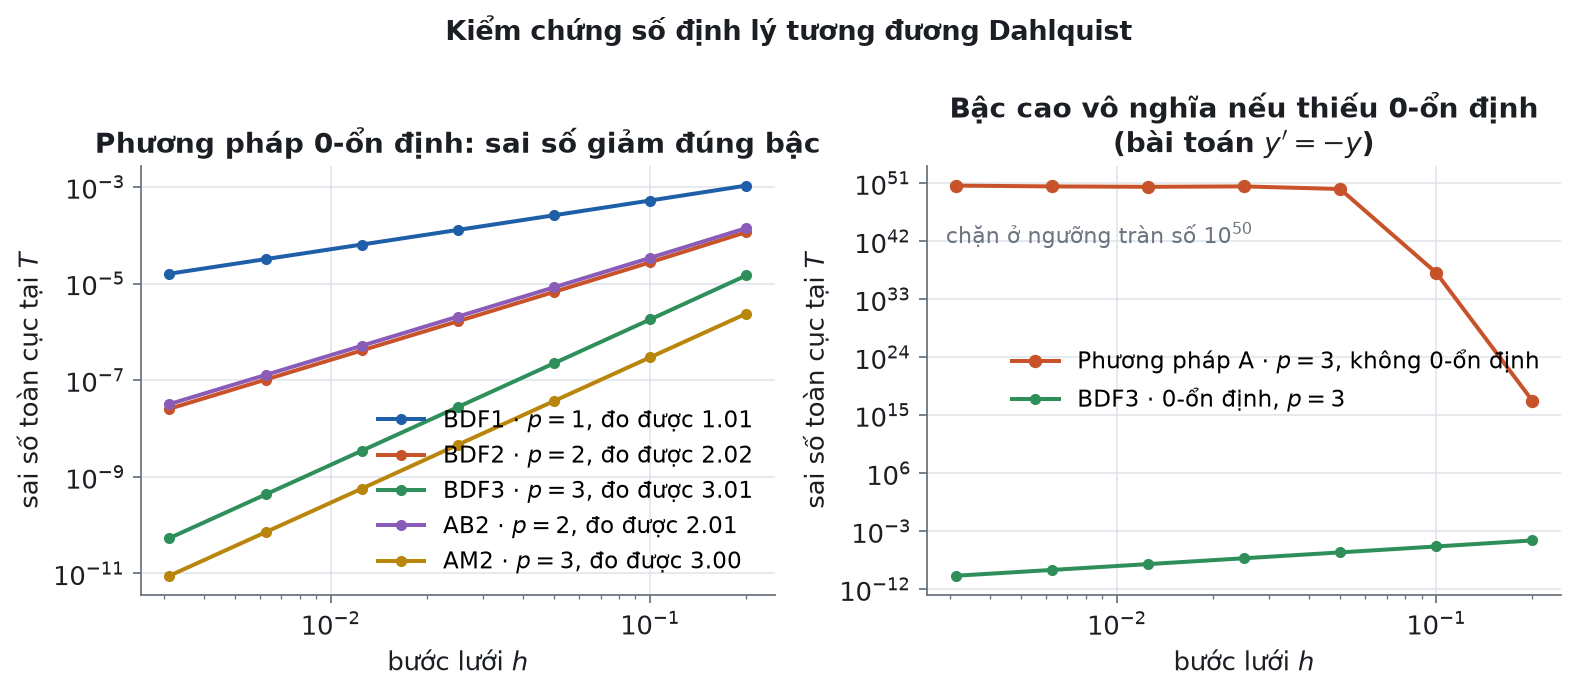
\includegraphics[width=0.92\textwidth]{../figures/fig04_convergence.png}
\end{center}
\vspace{-0.3em}
\footnotesize
Trái: năm phương pháp 0-ổn định trên $y'=y(1-y)$ — hệ số góc của $\log E$ theo $\log h$
đúng bằng bậc lý thuyết. Phải: BDF3 và phương pháp A \emph{cùng bậc $3$}, chỉ khác nhau
ở tính 0-ổn định.
\end{frame}

\begin{frame}{Sai số toàn cục: bậc lý thuyết so với bậc đo được}
\begin{center}
\scriptsize
% !!! TỆP NÀY ĐƯỢC SINH TỰ ĐỘNG — MỌI CHỈNH SỬA THỦ CÔNG SẼ BỊ GHI ĐÈ !!!
% Nguồn: code/experiments/ex07_report_tables.py  (chạy lại bằng: make figures)
\renewcommand{\arraystretch}{1.2}
\begin{tabular}{cccccc}
\toprule
$h$ & \textbf{BDF1} & \textbf{BDF2} & \textbf{BDF3} & \textbf{AB2} & \textbf{AM2}\\
 & $p=1$ & $p=2$ & $p=3$ & $p=2$ & $p=3$\\
\midrule
$0.2$ & $1.061\times 10^{-3}$ & $1.156\times 10^{-4}$ & $1.467\times 10^{-5}$ & $1.398\times 10^{-4}$ & $2.379\times 10^{-6}$\\
$0.1$ & $5.209\times 10^{-4}$ & $2.740\times 10^{-5}$ & $1.802\times 10^{-6}$ & $3.389\times 10^{-5}$ & $2.962\times 10^{-7}$\\
$0.05$ & $2.579\times 10^{-4}$ & $6.690\times 10^{-6}$ & $2.232\times 10^{-7}$ & $8.331\times 10^{-6}$ & $3.693\times 10^{-8}$\\
$0.025$ & $1.283\times 10^{-4}$ & $1.654\times 10^{-6}$ & $2.775\times 10^{-8}$ & $2.065\times 10^{-6}$ & $4.601\times 10^{-9}$\\
$0.0125$ & $6.396\times 10^{-5}$ & $4.114\times 10^{-7}$ & $3.455\times 10^{-9}$ & $5.138\times 10^{-7}$ & $5.684\times 10^{-10}$\\
\midrule
\textbf{bậc đo được} & $1.013$ & $2.032$ & $3.012$ & $2.021$ & $3.007$\\
\bottomrule
\end{tabular}

\end{center}
\vspace{0.4em}
\footnotesize
Mỗi lần giảm $h$ đi một nửa, sai số giảm $2^{p}$ lần. Sai lệch giữa bậc đo được và bậc
lý thuyết lớn nhất chỉ khoảng $0.03$.
\end{frame}

\begin{frame}{0-ổn định và ổn định tuyệt đối là hai chuyện khác nhau}
\begin{center}
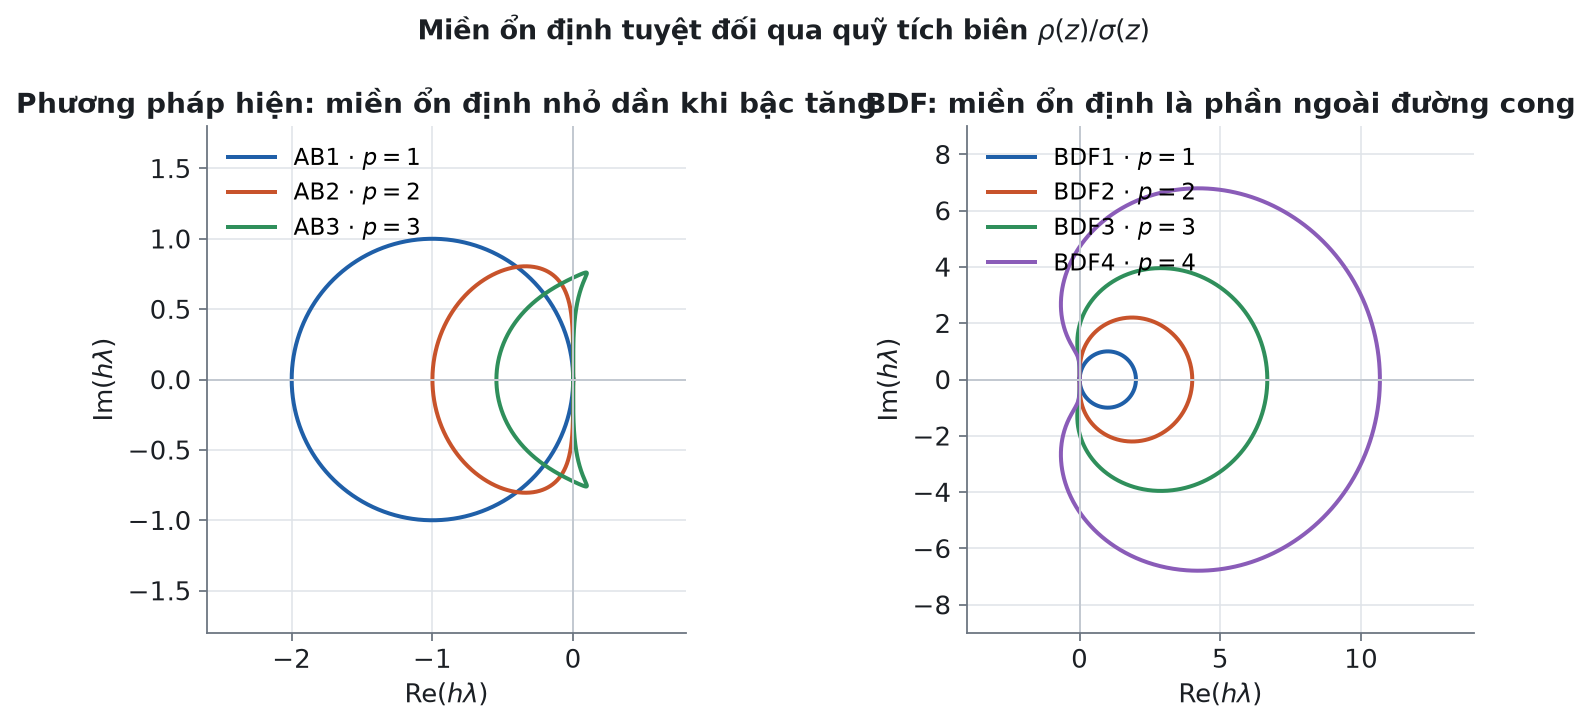
\includegraphics[width=0.92\textwidth]{../figures/fig05_stability_regions.png}
\end{center}
\vspace{-0.3em}
\footnotesize
AB3 vẫn 0-ổn định và vẫn hội tụ khi $h\to 0$, nhưng khoảng ổn định tuyệt đối của nó trên
trục thực âm chỉ là $(-6/11,\,0)$. BDF chứa toàn bộ trục thực âm, nên phù hợp với bài
toán cứng.
\end{frame}

% =========================================================
\section{Kết luận}

\begin{frame}{Tóm tắt}
\begin{enumerate}
  \item Phương pháp đa bước tuyến tính tận dụng nhiều giá trị quá khứ nên có hiệu quả tính toán cao.
  \item Tính nhất quán được kiểm tra bằng điều kiện
  \[
    \rho(1)=0,\qquad \rho'(1)=\sigma(1).
  \]
  \item Tính 0-ổn định được kiểm tra bằng điều kiện nghiệm của $\rho(z)$.
  \item Định lý Dahlquist cho biết:
  \[
    \text{Hội tụ}\Longleftrightarrow \text{Nhất quán} + \text{0-ổn định}.
  \]
  \item BDF nhất quán với mọi $k$, nhưng chỉ 0-ổn định với $k\le6$.
  \item Mọi kết quả trên đã được kiểm chứng bằng số: bậc hội tụ đo được khớp bậc lý
        thuyết, và $\max_i|z_i|$ của BDF vượt $1$ đúng từ $k=7$.
\end{enumerate}
\end{frame}

\begin{frame}{Tài liệu tham khảo}
\small
\begin{enumerate}
  \item K. Atkinson, W. Han, D. Stewart, \textit{Numerical Solution of Ordinary Differential Equations}, Wiley, 2009.
  \item E. Hairer, S. P. Nørsett, G. Wanner, \textit{Solving Ordinary Differential Equations I: Nonstiff Problems}, Springer, 1993.
  \item E. Süli, \textit{Numerical Solution of Ordinary Differential Equations}, Lecture Notes, University of Oxford, 2022.
\end{enumerate}
\vfill
\centering
\Large Cảm ơn thầy và các bạn đã lắng nghe!
\end{frame}

\end{document}
